\documentclass[twocolumn,letter]{vldb}
\special{papersize=8.5in,11in}

% comments
\newcommand{\mike}[1]{{\textcolor{green}{#1 -- MJF}}}
\newcommand{\joe}[1]{{\textcolor{red}{#1 -- JMH}}}
\newcommand{\minos}[1]{{\textcolor{cyan}{#1 -- MG}}}
\newcommand{\daisy}[1]{{\textcolor{magenta}{#1 -- DZW}}}
\newcommand{\sean}[1]{{\textcolor{blue}{#1--SLG}}}


% general
\renewcommand{\ttdefault}{cmtt}
\newcommand{\rbox}{\hfill $\Box$}

\newtheorem{thm}{Thorem}
\newtheorem{lem}{Lemma}
\newtheorem{ex}{Example}
\newtheorem{df}{Definition}[section]

\newcommand{\eat}[1]{}
\newcommand{\vpar}{\vspace*{.5em}}
\newcommand{\cut}[1]{}

\newenvironment{compactitemize}%
    {\begin{list}{}{
       \renewcommand{\makelabel}[1]{\bf $\bullet$}\hfil%
       \settowidth{\labelwidth}{\bf $\bullet$}%
       \setlength{\partopsep}{0mm}%
       \setlength{\parsep}{0mm}%
       \setlength{\parindent}{0mm}%
       \setlength{\itemsep}{0mm}%
       \setlength{\topsep}{0mm}%
       \setlength{\leftmargin}{\labelwidth}%
       \addtolength{\leftmargin}{\labelsep}
     }}%
    {\end{list}}

% BayesStore
\newcommand{\bs}{\textsc{BayesStore}\xspace}
\newcommand{\largebs}{{\large{\textsc{BayesStore}}}\xspace}
\newcommand{\Largebs}{{\Large{\textsc{BayesStore}}}\xspace}
\newcommand{\LARGEbs}{{\LARGE{\textsc{BayesStore}}}\xspace}
\newcommand{\hugebs}{{\huge{\textsc{BayesStore}}}\xspace}

% VLDB08 Abbreviations:
\newcommand{\ir}{$R$\xspace}
\newcommand{\sensor}{\textsl{Sensor1}\xspace}
\newcommand{\irset}{$\mathcal{R}$\xspace}
\newcommand{\pr}{\mbox{\sf Pr}}
\newcommand{\dom}{\mbox{\sf dom}}
\newcommand{\pdf}{$F$\xspace}
\newcommand{\true}{$true$\xspace}
\newcommand{\false}{$false$\xspace}
%\newcommand{\model}{$\mathcal{M}$}
\newcommand{\mv}{\textsl{miss}\xspace}
\newcommand{\RV}{\textsc{rv}\xspace}
\newcommand{\RVs}{\textsc{rv}s\xspace}
\newcommand{\bns}{\textsc{BN}s\xspace}
\newcommand{\mrfs}{\textsc{MRF}s\xspace}
\newcommand{\mrf}{\textsc{MRF}\xspace}
\newcommand{\rv}{$X$}
\newcommand{\pa}{$\mathcal{A}^p$\xspace}
\newcommand{\da}{$\mathcal{A}^d$\xspace}
\newcommand{\ed}{$\mathcal{ED}$}
%\newcommand{\entity}{e\xspace}
\newcommand{\es}{$\mathcal{E}$\xspace}
\newcommand{\op}{$\theta$\xspace}
%\newcommand{\bnf}{$\varphi$\xspace}
\newcommand{\fobnf}{$\phi$\xspace}
\newcommand{\fobn}{$\mathcal{M}_{FOBN}$\xspace}
\newcommand{\bn}{\textsc{bn}\xspace}
%\newcommand{\fbn}{$\textsc{fobn}$\xspace}
\newcommand{\MV}{$NULL$\xspace}
\newcommand{\mapping}{$f$\xspace}
\newcommand{\stripe}{$S$\xspace}
\newcommand{\selectivity}{\textsl{sel}\xspace}
\newcommand{\size}{\textsl{size}\xspace}
\newcommand{\missing}{\textsl{mratio}\xspace}
\newcommand{\connectivity}{\textsl{cratio}\xspace}
\newcommand{\probDB}{$\mathcal{DB}^p$}
%\newcommand{\exf}{$\mathcal{E}$}

% ICDE10

\newcommand{\tf}{text-string\xspace}
\newcommand{\IPD}{IPS\xspace}
\newcommand{\tfs}{text-strings\xspace}
\newcommand{\Tfs}{Text-strings\xspace}
\newcommand{\ie}{\textsc{ie}\xspace}
\newcommand{\model}{$\mathcal{M}$\xspace}
\newcommand{\tokenset}{\ensuremath{\mathbf{X}}\xspace}
\newcommand{\tokenseq}{\ensuremath{\mathbf{x}}\xspace}
\newcommand{\rvset}{\ensuremath{\mathbf{V}}\xspace}
\newcommand{\token}{\ensuremath{x}\xspace}
\newcommand{\labelset}{\ensuremath{\mathbf{Y}}\xspace}
\newcommand{\labelseq}{\ensuremath{\mathbf{y}}\xspace}
\newcommand{\crf}{$\mathcal{M}_{CRF}$\xspace}
\newcommand{\tokentbl}{\textsc{TokenTbl}\xspace}
\newcommand{\mr}{\textsc{MR}\xspace}
\newcommand{\strs}{$\mathcal{D}$\xspace}
\newcommand{\str}{\textit{d}\xspace}
\newcommand{\probsel}{\textit{probsel}\xspace}
\newcommand{\pwd}{\textit{pwd$(D^p)$}\xspace}

% HFGM-286report

\newcommand{\hfgm}{\textsc{hfgm}\xspace}
\newcommand{\rvs}{\textsc{rv}s\xspace}
\newcommand{\prm}{\textsc{prm}\xspace}

% extensibility

\newcommand{\pgm}{\textsc{PGM}\xspace}
\newcommand{\fctrset}{$\mathcal{F}$\xspace}
\newcommand{\probdbms}{\textsc{PDBMS}\xspace}

\newcommand{\argmax}{\operatornamewithlimits{argmax}}

\usepackage{times}
\usepackage{ams}
\usepackage{amsthm}
\usepackage{algo}
\usepackage{amsmath}
\usepackage{appendix}
\usepackage{graphicx}
\usepackage{xspace}
\usepackage{color}
\usepackage{subfigure}
\usepackage[small,compact]{titlesec}
%\usepackage{ulem} % Strikethrough font.
%\usepackage{abstract}
\usepackage[ruled,vlined]{algorithm2e}
\usepackage{balance}

\usepackage{balance}
\DeclareGraphicsExtensions{.pdf,.png,.jpg}

\title{CrowdPillar: Reducing Uncertainty in Probabilistic Databases by Leveraging Support from the Crowd}

\author{Sean Goldberg\\
	{\it University of Florida}\\
	%{\it\small Computer Information Science \& Enginnering}\\
	%{\it Gainesville, Florida}\\
	sean@cise.ufl.edu 
\and 
	Sunny Khatri\\
	{\it University of Florida}\\
	%{\it\small Computer Information Science \& Enginnering}\\
	%{\it Gainesville, Florida}\\
	skhatri@cise.ufl.edu 
\and
	Nilu Nalini\\
	{\it University of Florida}\\
	%{\it\small Computer Information Science \& Enginnering}\\
	%{\it Gainesville, Florida}\\
	nilu.nalini@gmail.com
\and 
	Daisy Zhe Wang\\
	{\it University of Florida}\\
	%{\it\small Computer Information Science \& Enginnering}\\
	%{\it Gainesville, Florida}\\
	daisyw@cise.ufl.edu
\and
	Tim Kraska\\
	{\it UC Berkeley}\\
	kraska@eecs.berkeley.edu}

\begin{document}
\maketitle

\begin{abstract}
The need to process and store large amounts of uncertain and imprecise data has necessitated the use of Probabilistic Databases (PDBs) which maintain and allow queries over data that carry a degree of uncertainty.  An integral part of the data cleaning process is finding efficient ways to reduce this uncertainty.  We propose CrowdPillar, a PDB system with an embedded graphical model structure that can employ crowdsourcing techniques such as Amazon Mechanical Turk (AMT) to resolve the most uncertain data entries.  CrowdPillar utilizes functions associated with the entropy over nodes in the graph to select which fields should be submitted to the crowd for correction.  This paper lays out the CrowdPillar system, discusses formulating questions for submission to AMT, and showcases the use of belief theory to combine responses for integration back into the PDB.
\end{abstract}


\section{Introduction}

Motivate need for automatic information extraction \newline

\noindent Discuss reasons for wanting to automatically segment citations \newline

\noindent Introduce system \newline

\noindent Briefly describe dataflow from extraction to selection and integration

% Motivate problem of uncertainty in database
% Machine learning methods have inherent uncertainty
% Goal is to reduce this uncertainty

\section{Background}

\subsection{Probabilistic Databases}

\subsection{Conditional Random Fields (CRF)}

\subsection{Inference Queries over a CRF Model}

\subsection{Uncertainty Sampling}

\subsection{Crowdsourcing}

% Probabilistic Databases
% Probabilistic Graphical Models
% Entropy
% Crowd

\section{System Overview}
\begin{figure}
\centering
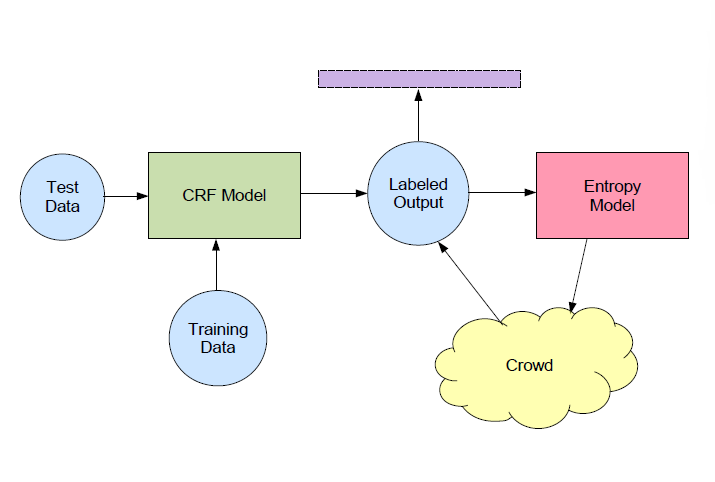
\includegraphics[width=0.9\linewidth]{images/system_design.png}
\label{fig:system_design}
\caption[example]{The CrowdPillar system design.  The top uncertain labeled outputs as determined by the entropy model are sent to the crowd.  The purple box denotes the specified application where the labeled data is ultimately sent.}
\end{figure}

The CrowdPillar system design is shown in \ref{fig:system_design}. The core of the system is designed as a modification to probabilistic databases that utilize PGMs as their data model.  Crowdpillar analyzes the uncertainty in the output and generates questions for crowd submission to reduce a Total Utility Function (TUF).  This is discussed in greater detail in Section 4.  The response of the crowd is combined in a principled way with the original PGM output using Dempter-Shafer belief theory, as described in Section 5.

In this paper we consider a sample application task and follow it through the major components of the system: the probabilistic database, question formulation, crowd submission, and data fusion.

Consider an extraction system for automatically reading published citations and storing them in the database.  In order to fit an incoming citation into any nontrivial schema, the string has to be appropriately chunked to determine which tokens belong to which attributes.  A string such as:
\begin{quotation}
\textit{Perfect Model Checking via Unfold/Fold Transformations. Maurizio Proietti, Alberto Pettorossi CL 3-540-67797-6 Springer Lecture Notes in Computer Science Computational Logic - CL 2000, First International Conference, London, UK, 24-28 July, 2000, Proceedings 2000}
\end{quotation}
needs to be labeled with its appropriate title, author, conference, etc.  This is in general a nontrivial problem, especially when one considers the numerous styles and orderings different citations come in.  An efficient extraction system must be trained to handle these different occurences.

The state of the art model for this type of information extraction task is the conditional random field.  We focus specifically on CRFs for the remainder of the paper and make it the flagship example of CrowdPillar, though there exist other models that can derive the appropriate labelings and confidences for which CrowdPillar would also apply.  After the CRF has segmented and labeled the data, each label sequence is stored as a possible world as in Figure (\ref{fig:CRFexample}b)

The goal of CrowdPillar is to optimally select a number of sequences of high uncertainty from the CRF output and query the crowd for the label of each token in a sequence with the highest individually assigned score.  We discuss specifically how scoring is done in Section 4 and how many questions can be asked depends on the user's cost and time budget.  An on-line approach to selecting sequences is highly inefficient due to the relatively slow speed of returning a crowd response (on the order of hours) as well as the high parallelizability of largely independent sequences.  For these reasons, sequences are selected in a batch for submission to the crowd.

After determining which sequences should be sent, we generate a question in XML format for each sequence.  Questions may be in the form of multiple choice, fill in the label, yes/no, etc.  Given the possible uncertainty in the crowd response, we resolve conflict and combine multiple answers to each question using Dempster-Shafer belief theory based on a quality metric attached to each answer to ultimately generate a probabilistic collection of responses to each question.  The quality $Q\rightarrow[0,1]$ may take a number of different forms, including difficulty of the question and approval rating and bias of the responder.  It represents the confidence we have in the answer being correct as opposed to being a randomly generated guess.

The crowd submissions are sent back to the PDB upon completion, where they are combined with the original output CRF data using the Dempster-Shafer Theory of Evidence.  The answers can be returned at once upon completion of the batch or queried in intervals.  How often to specifically query for answers will be dependent on the user's specifications and needs. 


% System Overview and Components

\section{Question Formulation}
Given a graphical model designed to perform statistical analysis upon a PDB and the uncertainty associated with a set of unobserved nodes, the main task of CrowdPillar is designating which nodes to observe and by performing inference reduce the uncertainty of the entire system.  Observation is the act of clamping a random variable to a specific value.  For the case of information extraction, this is label provided by the crowd.

This section is concerned with precisely how to select the optimal node to observe from a graphical model.  The node whose resolution best reduces the overall model uncertainty is the one sent to the crowd.  Before we can form a discussion about optimal node selection, we must first introduce the metric by which uncertainty is measured in our sysem.

\subsection{Total Utility Function}
In order to make a decision about which node to query, we develop the concept of a Total Utility Function (TUF). The TUF fulfills two prominent and necessary roles: quantification and selection.  At its core, it represents a quantification of the uncertainty so that we may measure differences in total uncertainty between different configurations of our model.  The second functionality is that is designed in such a way as to rapidly promote uncertainty reduction by identifying the key node hubs whose resolution gives the greatest effect.  Node features such as entropy and dependency need to be taken into account and will be discussed in greater detail later in the section. 

There are two paradigms that may be used here.  The first is to assign each node $t$ a score $S_{t}$ in a simple manner and combine them in some complex model-dependent way.  The other is to leave the score combination simple. but create complex ways to attach a score to each node.  We choose the latter approach because it is more easily generalizable to various PGMs.

The simplest way to combine scores is to take the sum, ie. for a model with T nodes:
\begin{equation}
TUF = \sum_{t=1}^{T}S_{t}
\end{equation}
This makes node selection for uncertainty reduction simple.  By observing the node with the highest score and reducing that score to zero, the entire function is maximally reduced.  The tradeoff is that the method of assigning a score may be much more complex.  We devote the remainder of this section to discussion of the various techniques for assigning a score and settle on a combined metric that we assert can be used for a wide range of probabilistic graphical models.

\subsection{Simple Methods of Assigning Scores}
Below we present two methods of attaching scores to nodes based on their marginal entropy and dependency among other nodes.  The main application of these methods is to linear-chain conditional random fields, but additional model dependent methods may be used in the appropriate context.  

\subsubsection{Marginal Entropy}
Linear-chain Hidden Markov Models or Conditional Random Fields are one the simplest type of PGM to assign a score to due to the uniformity of each node in the graph.  With the exception of the first and last nodes in the chain, every node has the same type and number of pair-wise edge features.  Thus any means of assigning $S_{t}$ is consistent across all nodes.

The property we hope to achieve with score assignment is to give the largest scores to the most uncertain nodes.  The uncertainty associated with a specific node is achieved by calculating the entropy over its marginalized distribution.  Marginalization in a CRF is done through the forward-backward algorithm \cite{Lafferty01} utilizing forward ($\alpha$) and backward ($\beta$) inference messages meeting at the marginalized node.  The marginal probability of a node $t$ in the sequence being assigned label $i$ is given by
\begin{equation}
p(\mathbf{Y}_{t}=y_{i}|\mathbf{x}) = \frac{\alpha_{t}(y_{i}|\mathbf{x})\beta_{t}(y_{i}|\mathbf{x})}{Z(\mathbf{x})}.
\end{equation}
The marginal entropy of node $t$ is then
\begin{equation}
H_{t} = \sum_{i=1}^{L}p(\mathbf{Y}_{t} = y_{i}|\mathbf{x})log[p(\mathbf{Y}_{t} = y_{i}|\mathbf{x})],
\end{equation}
where L is the label space of the problem.  This leads to a simple uncertainty score assignment of $S_{t}=H_{t}$.

In making a decision about which node in a sequence of length $T$ to the submit to the crowd, we calculate the marginal entropy $H_{t}$ for every node and take the highest one,
\begin{equation}
Selection = \argmax_{t}(H_{t}) \hspace{0.5in} t=1,\dots,T.
\end{equation}
The crucial assumption here is that the most uncertain node generally has the highest probability of being incorrect compared with other nodes in the sequence.  In our experiments in Section 6 we show that this is a safe assumption to make.  

Although the response from the crowd only holds information pertaining to a single node's assignment, inference provides a wider-reaching chain reaction effect.  As discussed earlier, the most likely path sequence is determined by a type of Viterbi dynamic programming algorithm.  After clamping the label of node $t$ to label $i$, we run a Constrained Viterbi \cite{Kristjansson:2004:IIE:1597148.1597216} which fixes the Viterbi path to run through $i$ at $t$.  This may change the labels of other nodes in $t$'s neighborhood compared to before clamping.  Thus the total entropy of the entire sequence may be reduced well beyond the contribution of the selected node.

\subsubsection{Most Dependency}
Since inference provides a means of updating multiple nodes from a single answer, it would be useful to have a score that is proportional to this chain reaction effect.  That is, those nodes with the greatest ability to impact its surrounding neighborhood should be awarded the highest score.  This increases the impact of every question asked. 

For generalized graphical models, it is clear the impact of resolving a node is proportional to the number of nodes which share edge-wise features with it.  Nodes with a higher degree are more "important" to resolve.  Thus another metric for scoring can be the degree of each node,
\begin{equation}
SELECTION = \argmax_{t}(deg(V_{t})) \hspace{.2in} t=1,\dots,T.
\end{equation}

To illustrate this idea further, consider an experiment involving a connected social network and movie recommendation system.  We want to select a single user to ask about which movies they like and in turn make recommendations to their friends under the assumption that friends like similar movies.  The user likely to give the maximum number of recommendations is simply the one with the most friends.  Modeling the social network as a graph, this is the node with the most connections.

This score assignment based on the node with the highest dependency can also be used in the information extraction domain.  One recent modification to the linear-chain model is to use "skip-edges" \cite{Sutton04} connecting possibly distant nodes in the sequence.  The goal is for multiple nodes representing the same entity to be resolved simultaneously.  In this case we would seek to ask a question about the nodes connected by the greatest number of skip-edges, ie. resolving those entities that appear most in the sequence and whose resolution has the greatest impact.

\subsection{Neighborhoods: Total Score Metric}
It is desirable to be able to assign a score to a a node in a generalized probabilistic graphical model without explicitly depending on the type of model, eg. linear-chain vs. skip-chain.  The two factors by which a score can be measured are the entropy of the node and its degree.  To this end, we propose a method that combines both properties and can be applied to a numerous models more general than the linear-chain discussed in detail in this earlier in this section.

\begin{figure}
\centering
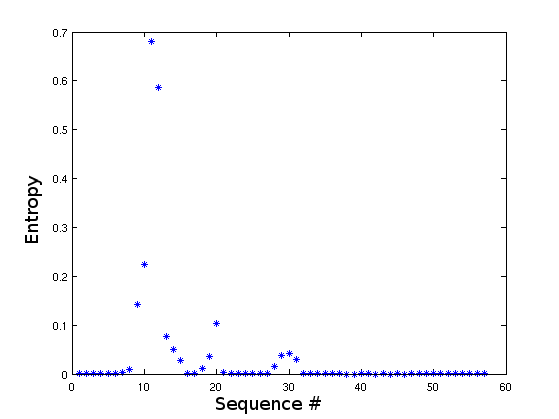
\includegraphics[width=0.9\linewidth]{images/ent_dist1.png}
\label{fig:ent}
\caption[example]{The entropy distribution for a sample bibliographic sequence.}
\end{figure}

Figure \ref{fig:ent} shows the entropy distribution for the labeling of a sample bibliographic sequence.  Rather than being randomly distributed, high entropy values appear in pockets of small neigborhoods.  This is standard among many sequences investigated.  This notion of clustering of high entropy nodes around the highest ones in the sequence motivates an additional method of combining scores that naturally carries the properties needed from the previous two sections.

Instead of taking the marginal entropy over a single node as the only score metric, we combine the entropies of each node with those of all nodes of order $K$ or less.  By this we mean all nodes connected to the node in question by $K$ or fewer edges.  Formally:
\begin{multline}
S_{t} = \sum_{i=1}^{L}p(\mathbf{Y}_{t} = y_{i})log[p(\mathbf{Y}_{t} = y_{i})]\\
+\sum_{k=1}^{K}\sum_{j=1}^{L}p(\mathbf{Y}_{t+k} = y_{j})log[p(\mathbf{Y}_{t+k} = y_{j})]\\
+\sum_{k=1}^{K}\sum_{m=1}^{L}p(\mathbf{Y}_{t-k} = y_{m})log[p(\mathbf{Y}_{t-k} = y_{m})]
\end{multline}
In our experiments we take $K=1$ and analyze all nodes connected by a single edge.  Again $SELECTION$ is the node with the max $S_{t}$.

As per Figure \ref{fig:ent}, this should have little effect on the single highest marginal method for linear-chain models.  The highest entropy node in a sequence usually appears among other high entropy nodes.  In addition, for models with greater variation in connectivity, nodes with a larger neighborhood will generally have a larger score by the Neighborhood Metric.  This method automatically accounts for the tradeoff between node pockets of high entropy and others that are connected to a larger number neighboring nodes.  Currently, we only cover linear-chains CRFs, but we plan to apply this method and conduct experiments on other models such as Bayesian Networks in our future work.

% Total Utility Function
% Assigning Scores to Nodes
%   Highest Marginal
%   Most Frequent
%   Most Dependency
% Combined metric


\section{Probabilistic Data Integration}

While the previous section focused on the number of ways to select a node in a PGM to submit to the crowd, it remains to be seen how to handle the retrieved result.  The problem is handled as a task in probabilistic data integration involving data from both the machine model and the crowd.  In this section we discuss a method of combining crowd response and integrating it back into the system in a probabilistic manner.

\subsection{Uncertainty From the Crowd}
In an ideal world, all the responses coming from the crowd will be correct values equivalent to the ground truth.  We formulate a question, get an answer, and replace fields that were requested.  In practice, there are numerous reasons a single person from the crowd may not supply the correct result.

Services like Amazon Mechanical Turk are subject to spammers that provide random responses in order to reap the benefit of a Human Intelligence Task (HIT) while doing little of the actual work \cite{Panos10}.  A good deal of research has been done to reduce the effect of spammers including repeated labeling \cite{Sheng:2008:GLI:1401890.1401965} and interspersing ground truth to gauge Turker effectiveness \cite{quinn10}.  Even honest Turkers, however, may not always give the correct response for reasons such as lack of knowledge, inexperience, or increased difficulty of the questions.  The golden standard has been to ask the question multiple times and take a majority vote among the users. 

Here we model a new way of looking at the crowd response, viewing it as an application of probabilistic data integration.  In traditional data integration, data is combined from multiple heterogeneous sources to give the user a single, unified view.  Probabilistic data integration attaches probabilities to the combined result.  Generally, there is ambiguity in the compatibility of certain relations which leads to a probability value as a result of combination itself, despite the data being indivudally deterministic.

It's also possible for the data coming from different sources to include probability as a first class citizen, that is, the data is naturally probabilistic, such as the combination of probabilistic sensor data.  Combining results from the crowd becomes an application in probabilistic data integration if we take each Turker to be a source of data and attach probabilities to their answers based on some quality rating.  This quality rating can be something simple like the Turker's approval rating or something more complex.  For instance, Panagiotis et al. \cite{Ipeirotis:2010:QMA:1837885.1837906} build upon a model for recovering worker error rates by Dawid and Skene \cite{dawid79} and are able to separate worker bias to assign a true Turker accuracy.

We employ the machinary of the Dempster-Shafer model of belief functions to combine probabilistic evidence from multiple workers.  The goal is to combine data to present a single unified crowd response for merging with the original CRF output in the PDB.  This second step of combining crowd and CRF can be accomplished using the same method, but treating the total crowd and CRF as different probabilistic sources.

\subsection{Dempster-Shafer Belief Model}
The Dempster-Shafer (DS) model \cite{dempster67a, Shafer76} employs a mathematical object called a belief function that measures the degree of belief (or mass) someone has about an event.  The uncertainty associated with a belief corresponds with missing or incomplete data, as opposed to fuzzy or possibilistic data.  Collecting evidence from different sources, one can establish a degree of belief about the reliability of the source itself and therefore also the evidence presented.

Consider an event $X$.  Dempster-Shafer theory maps each element of the power set of $X$ to the interval $[0,1]$.  This mapping is referred to as the \textit{mass function}.  The fundamental properties of the mass function are:

\begin{equation}
m(\emptyset) = 0
\end{equation}
\begin{equation}
\sum_{A\in2^{X}} m(A) = 1
\end{equation}

That is, the mass of the empty set is always zero and the remaining members of the power set have to sum to 1.

To motivate back to our original problem of information extraction, let's assume binary labelings for a token, $X=\{0,1\}$.  Of the four elements of the power set of X, only 3 have mass functions: $m(\{0\})$, $m(\{1\})$, and $m(\{0,1\})$.  They correspond to the mass that the proper label is 0, that the proper label is 1, or that we are uncertain and the proper label can still be either 0 or 1.

The \textit{belief} in a set is the sum of all elements of the power set that contain that set.  Therefore the belief in label 0 is defined as $m(\{0\})+m(\{0,1\})$, with a similar function for the belief in label 2.  Renormalizing over the beliefs provides a probability distribution over the set of labels.

Mass functions from multiple sources may be combined in a principled manner using Dempster's Rule of Combination.  Let's presume we have two different mass functions $m_{0}$ and $m_{1}$.  The \textit{joint mass} is found with:

\begin{equation}
\begin{split}
m_{0,1}(\emptyset) &=0\\
%\end{equation*}
%\begin{equation*}
%\begin{split}
m_{0,1}(A) &=(m_{0}\oplus m_{1})(A)\\
                   &=\frac{1}{1-K} \sum_{B\cap C=A\neq\emptyset} m_{0}(B)m_{1}(C)
\end{split}
\end{equation}

where

\begin{equation}
K=\sum_{B\bigcap C=\emptyset}m_{0}(B)m_{1}(C)
\end{equation}

The combination is essentially a normalized outer product.  All combinations with an intersection equal to the event in question are summed.
 
\subsection{Combining Crowd Data}

If multiple Turkers are treated as different sources and their responses as evidence, we can map those responses to belief functions and combine them using the Rule of Combination.  The usual technique is to ask the same question to multiple Turkers and take a majority vote.  While generally effective, there arise situations where the crowd is split on a result.  Possibilities include an image of poor quality or a text analytic question in which the majority of workers are not proficient in English \cite{Rashtchian:2010:CIA:1866696.1866717}.

Let's say that we limit responses to only those Turkers with a 75\% quality rating (that is, they give the correct label 75\% of the time and an incorrect label 25\% of the time) or above and do a best of 5 majority vote.  If three Turkers with an approval rating of 75\% answer label  and two turkers with an approval rating of 100\% answer label 1, the majority vote takes label 1 and passes no other information about who responded with which label.  If a particularly difficult question has Turkers divided, such uncertainties can not be stored and processed in a traditional DB.  Our use of a PDB framework allows the uncertainties to persist and the combination method provides a more reliable estimate of this uncertainty. 

If the crowd gives conflicting  responses to a question, this discrepancy can be reflected within the database by determining the belief we have that each answer is correct.  This is where we make use of the machinery of Dempster-Shafer theory.  For each question submitted, we maintain a running mass function for the correctness of each possible answer.  This function is updated as new responses come in from the crowd.  If there are $n$ possible answers, we are concerned with $n+1$ masses, one for each answer plus the uncertainty mass that the Turker is unreliable and their response is equivalent to a random answer.  


\begin{algorithm}
	\SetAlgoLined
	\KwData{Question $Q$, Turker $T$, Response $R \in [1,n]$}
	\KwResult{$Q.m =$ Total mass for Q}
	\Begin{
		$n \equiv$ number of possible answers to $Q$\;
		$Q.m \equiv$ current mass for Q\;
		Initialize masses $m[1]$,...,$m[n+1]$ to $0$\;
		\tcp{Map response and uncertainty to mass functions}
		$m[R] \leftarrow T.rating$\;
		$m[n+1] \leftarrow 1-T.rating$\;
		\tcp{Check if this is the first response}
		\eIf{$Q.m =$ NULL}{
			\Return{$Q.m \leftarrow m$}		
		}
		{
			Initialize $sum[1]$,...,$sum[n+1]$ to $0$\;
			\For{$p=1$ \KwTo $n+1$}{
				Initialize $K \leftarrow 0$\;
				\For{$i=1$ \KwTo $n+1$}{
					\For{$j=1$ \KwTo $n+1$}{
						\tcp{Take outer product}
						$Outer \leftarrow m[i]*Q.m[j]$\;
						\tcp{Check for intersection}
						\eIf{$i=j$ or $i=n+1$ or $j=n+1$}{
							$sum[p] \leftarrow sum[p]+Outer$\;
						}
						{
							$K \leftarrow K+Outer$\;
						}
					}
				}
				\tcp{Renormalization}
				$sum[p] \leftarrow (\frac{1}{1-K})*sum[p]$\;
			}
			\Return{$Q.m \leftarrow sum$}
		}
	}
	\caption{Update Answer Belief}
	\label{DSCombo}
\end{algorithm}

Algorithm \ref{DSCombo} displays the pseudocode for updating a question's current mass function with a new response provided by the Turker. We assume the response takes the form of a multiple choice answer and ranges from $1$ to $n$.  The mass function associated with the Turker is zero for every answer except the one they chose, which gets mapped to their quality rating in $[0,1]$.  This defines the likelihood they picked the correct answer.  Their unreliability gets mapped to the set of all possible answers $m[n+1]$.

If there is no current mass associated with the question, the current Turker mass is taken as the Question's mass.  Otherwise, we need to combine the two masses using Dempster's Rule of Combination.  Remember that the combination for each answer is an outer product over all sets that have an intersection equivalent to that answer.  Here we assume mutual exclusivity among all choices and so this intersection occurs only when $m$ and $Q.m$ are the same answer or either is the set of all possible answers.  The final result is a newly combined mass function which can easily be converted into a probability distribution for that question and integrated back into the PDB.

\subsection{Combining Crowd and Machine}

After combining multiple answers from the crowd, the total crowd response needs to be aggregated with the original graphical model output.  One method is to completely eliminate the machine response and simply put the crowd data in its place.  Given the increased reliability of human authors, this can lead to desirable results.

We take a differing view, however, like a detective collecting evidence from different sources.  The PGM and crowd represent merely two different sources from which conclusions are being drawn.  Rather than throwing away information, we seek to ML and crowd answers in the same principled way.  On questions in which the crowd is divided amongst itself, we can use the original PGM to "break the tie".

The combination of crowd and machine is the same as Algorithm \ref{DSCombo}, except that that there exists no analog to the quality rating in the machine output.  While a confidence value can be attributed to a measure of certainty, it is not necessarily true that the complement is a measure of randomness.  The simple method is to forego the use of a quality rating and uncertainty metric and map the confidence values for each label directly to its associated mass function.  The label confidence from a CRF can be attributed from the marginal probabilities \cite{Kristjansson:2004:IIE:1597148.1597216}. 

The final result is a complete mass function which can easily be converted into a probability distribution.

% Combining probabilities from multiple models.
% Dempter-Shafer belief theory

\section{Experiments}
In this section we demonstrate the effectiveness of our selection and integration approaches on sets of both synthetic and real data.  We extracted 14,000 labeled citations from DBLP \sean{footnote 1} and 500,000 from the PubMed database \sean{footnote 2}.  For unlabeled testing data, we removed the labels and concatenated text from each of the available fields.  Order of fields was occasionally mixed in keeping with real-life inconsistency of citation structure.

\subsection{Experiments w/ Synthetic Data}
\subsubsection{Selection}

\begin{figure*}[t]
	\centering
	\subfigure[High Entropy] {
		\includegraphics[width=0.48\textwidth]{images/selection_exp1_highE.png}
		\label{fig:first1}
	}
	\subfigure[Total Entropy] {
		\includegraphics[width=0.48\textwidth]{images/selection_exp1_totalE.png}
		\label{fig:second1}
	}
	\caption{Seeding comparison for high entropy and total entropy ranking.}
	\label{fig:select1}
\end{figure*}

\begin{figure*}
	\centering
	\subfigure[High Entropy] {
		\includegraphics[width=0.48\textwidth]{images/selection_exp2_highE.png}
		\label{fig:firs2t}
	}
	\subfigure[Total Entropy] {
		\includegraphics[width=0.48\textwidth]{images/selection_exp2_totalE.png}
		\label{fig:second2}
	}
	\caption{Clustering comparison for high entropy and total entropy ranking.}
	\label{fig:select2}
\end{figure*}

\begin{figure*}
	\centering
	\subfigure[High Entropy] {
		\includegraphics[width=0.48\textwidth]{images/selection_exp3_highE.png}
		\label{fig:first3}
	}
	\subfigure[Random] {
		\includegraphics[width=0.48\textwidth]{images/selection_exp3_random.png}
		\label{fig:second3}
	}
	\caption{Ranking comparison for high entropy and total entropy ranking.}
	\label{fig:select3}
\end{figure*}

Figures~\ref{fig:select1},~\ref{fig:select2}, and~\ref{fig:select3} contain experiments comparing our various selection algorithms by detailing the accuracy improvements for each question asked.  Tokens were selected using a specific combination of seeding, clustering, and ranking approaches.  

Initially, a token was selected from each document using some seeding mechanism.  The number of questions is prohibitively large to show the full range of our methods, so we automatically answer each question with its ground truth label.  It's shown in the next section that the high accuracy of Mechanical Turk answers allow this to be a working assumption.  The same answer (label) to the question (token) is applied to all subsequent tokens in its cluster.  A constrained Viterbi inference algorithm runs over all documents  containing tokens belonging to question clusters.  The accuracy value in each figure represents the final token accuracy after running constrained inference.

In this paper, we proposed two possible functions for selecting a token from each document.  High Entropy chooses that which has the highest marginal entropy over its labels while Neighborhood Entropy selects the token in the center of the largest 3-window pocket of marginal entropies.  Figure~\ref{fig:select1} shows effectiveness of both methods when compared to randomly selecting a token for both High Entropy and Total Entropy ranking.  The default clustering is Same Label Neighborhood.  In both cases, Neighborhood Entropy maintains a consistently higher accuracy, lending evidence to the idea that constrained inference has a larger effect on pockets of high entropy than it does on the single highest entropy tokens.  Both methods double the overall possible accuracy improvement with fewer questions.  For some accuracy regions even orders of magnitude fewer questions are needed.

Figure~\ref{fig:select2} compares the possible clustering algorithms for the High Entropy and Total Entropy ranking functions.  All use high entropy for seeding.  Clustering by similar tokens that have the same label and share preceding and succeeding labels produce the largest clusters with the greatest net effect.  For the DBLP set, there were zero clustering errors for Same Token and Same Field, and approximately 2\% of citations were clustered incorrectly using the Same Label approach.  As the figures prove, however, the benefit of larger clusters far outweigh the additional errors.

The final set of synthetic selection experiments is shown in Figure~/ref{fig:selection3}.  While it initially seemed like a heuristic, the effectiveness of Total entropy for ranking should now be apparent.  For both high entropy and random seeding, total entropy combines the early question strength of large clusters and the late question power of high entropy.  Same Label Neighborhood is again the default clustering for all ranking comparisons.  It's important to note, that even for random seeding, Total Entropy outperforms everything else.



\subsubsection{Integration}
\begin{figure}
		\includegraphics[width=0.48\textwidth]{images/integration_exp1_numT.png}
		\label{fig:integrate1}
		\caption{Comparison of integration methods vs. number of Turkers per question.} 
\end{figure}
\begin{figure}
		\includegraphics[width=0.48\textwidth]{images/integration_exp2_meanQ.png}
		\label{fig:integrate2}
		\caption{Comparison of integration methods vs. average Turker quality.} 
\end{figure}

Answers received from the crowd have many variables that must be factored into a rigorous justification of any method of combination.  Primarily, we are concerned with measuring how the final combined accuracy is affected both by the number of redundant answers and by the actual quality of the workers.  A set of synthetic responses to real questions were generated in a manner that the allowed the average worker quality to be varied throughout the experiments.

Workers were automatically generated by selecting a quality value $Q \in [0,1]$ from a Gaussian distribution of standard deviation 0.3 and a mean that varies over the experiment.  Quality values drawn outside the $[0,1]$ range were truncated at the boundary.  Each worker was assigned to a 'HIT', which constituted a set of 10 questions.  The quality level dictated the generation of answers.  In keeping with our assumption of quality, the true label was applied with probability $Q$.  With probability $1-Q$, the answer was drawn from a uniform distribution over the label space.  In this manner we assembled 500 questions answered by 3-13 workers each, with new sets of workers generated every 10 questions.

Figure~\ref{fig:integrate1} shows how the integration methods outlined in this paper compare as we increase the redunancy of question asking.  The mean worker accuracy is 0.5 in these results and the prior used in the Bayesian method is uniform.  While all methods increase monotonically as expected, the Bayesian method produces the best results for low redundancy and both Bayesian and Dempster-Shafer are able to attain 100\% accuracy by 13 workers, whereas Majority Voting is not.  The Bayesian method is able to beat Dempster-Shafer slightly due to its uniform prior assumption, which closely follows the distribution of labels for low quality workers.

The availability of high or low quality workers is certain to affect the comparisons, so in Figure~\ref{fig:integrate2} we compare the accuracy of answers as we vary the quality.  Variation is achieved by shifting the center of the Gaussian which produces worker quality values.  We initially set it at 0.2 and shifted to a maximum of 0.8.  As before, the Bayesian and Dempster-Shafer approaches show that managing Turker quality, even when so low as to be just slightly better than random, produces large gains in accuracy.  One method of attaining only high quality workers on Amazon Mechanical Turk is to implement a qualification test that workers must pass before they can complete your tasks.  Our experience has shown that while this does lead to more abled workers, the price paid in time can be many times slower.  The results of Figures~\ref{fig:integrate1} and~\ref{fig:integrate2} show that with a better integration method, some of the constraints designed to achieve higher quality may be relaxed without a large decrease in accuracy, key to making \sysName fast, agile, and powerful.

\sean{Exp6: Recall vs. accuracy for varying entropy thresholds.}

\subsection{Experiments w/ Real Data}
\sean{Description of real experiment methodology.}

\sean{Exp7: Table of accuracy comparisons for DS, MV, and Bayes before and after edits plus clamped inference for both data sets.}

\sean{Exp8: Recall vs. accuracy for varying entropy thresholds for both data sets.}

% Overview of experiments conducted.

%\section{Future Work}


\section{Conclusion}
\balance

\balance
%\begin{thebibliography}{9}

\bibitem{dempster67}
Arthur P. Dempster: \textit{Upper and Lower Probabilities Induced by a Multivalued Mapping}. Classic Works of the Dempster-Shafer Theory of Belief Functions 2008: 57-72.

\bibitem{shafer76}
Glenn Shafer: \textit{A Mathematical Theory of Evidence}, Princeton University Press, 1976, ISBN 0-608-02508-9.

\bibitem{crowdfllow}
Alexander J. Quinn, Benjamin Bederson, Tom Yeh, Jimmy Lin, \textit{Crowdflow: Integrating Machine Learning with Mechanical Turk for Speed-Cost-Quality Flexibility}, Technical Report HCIL-2010-09, University of Maryland, 2010

\bibitem{lafferty}
J. Lafferty, A. McCallum, and F. Pereira. \textit{Conditional random Fields: Probabilistic models for segmenting and labeling sequence
data}. In Proc. ICML-01, pages 282–289, 2001.
\end{thebibliography}
\bibliographystyle{abbvr}
\bibliography{citation}

\end{document}
